\documentclass[12pt]{article} 
\usepackage{amsmath} 
\usepackage[dvips]{graphicx}
\usepackage{multirow} 
\usepackage{geometry} 
\usepackage{pdflscape}
\usepackage[labelfont=bf]{caption} 
\usepackage{setspace}
\usepackage[running]{lineno} 
% \usepackage[numbers,sort]{natbib}
\usepackage[sort]{natbib} 
\usepackage{array}
\usepackage[table]{xcolor}
\usepackage{xr}

\newcommand{\methods}{\textit{Materials \& Methods}}
\setcounter{section}{0}
\renewcommand{\thesection}{S\arabic{section}}
\setcounter{table}{0}
\renewcommand{\thetable}{S\arabic{table}}%
\setcounter{figure}{0}
\renewcommand{\thefigure}{S\arabic{figure}}%
\setcounter{equation}{0}
\renewcommand{\theequation}{S\arabic{equation}}
\renewcommand{\labelenumi}{S\arabic{enumi}}


\topmargin -1.5cm % 0.0cm 
\oddsidemargin 0.0cm % 0.2cm 
\textwidth 6.5in
\textheight 9.0in % 21cm
\footskip 1.0cm % 1.0cm

\usepackage{authblk}

\begin{document} 

\title{Species motif participation provides unique information about species risk of extinction}

\author{Alyssa R. Cirtwill$^{1*\dagger}$, Anna \r{A}kesson$^{2*}$, Kate L. Wootton$^{3}$, Anna Ekl\"{o}f$^{2}$} 
\date{
\small$^1$Spatial Foodweb Ecology Group\\
Research Centre for Ecological Change\\
Organismal and Evolutionary Biology Research Programm\\
Faculty of Biological and Environmental Sciences\\
University of Helsinki, Helsinki, Finland\\
\medskip
\small$^2$Department of Theoretical Biology, Chemistry, and Physics\\ 
Link\"{o}ping University, Link\"{o}ping, Sweden\\
\medskip
\small$^3$ BioFrontiers Institute\\
University of Colorado, Boulder, Boulder, U.S.A.\\
\medskip
* Joint first authors\\
\medskip
$^\dagger$ Corresponding author\\
}


\maketitle 
\raggedright

\setlength{\parindent}{15pt} 
\begin{spacing}{2.0}

\clearpage

\section*{Table of contents}
    {\footnotesize
    \begin{spacing}{1.0}

    Appendices S1-S3 provide supplemental methods, while appendices S4-S8 provide supplemental results.

    \begin{enumerate}
    
        \item Calculating persistence

            \begin{itemize}
                \item Details on functional response of consumers
                \item Contains Eqn. S1
            \end{itemize}    
            

        \item Network creation \\
        
            \begin{itemize}
            \item Construction of simulated networks
            \item Filtering of biologically unrealistic networks 
            \item Conversion of networks to acyclic form
            \item Comparison of empirical and simulated networks
            \end{itemize}
            
            
        \item Statistical analysis

            \begin{itemize}
                \item Species persistence and motif participation (Eqn. S2-3)
                \item Motif participation and network properties (Eqn. S4-6)
                \item Network mean persistence and motif profiles (Eqn. S7)
                \item Network motif profiles and global network structure (Eqn. S8)
                \item Persistence and other network properties (Eqn. S9-11)
            \end{itemize}
                

        \item Persistence and motif participation
            \begin{itemize}
                \item Contains Table S1
            \end{itemize}


        \item Participation and network properties

            \begin{itemize}
                \item Contains Table S2
                \item Contains Fig. S1
            \end{itemize}
    
        \item Persistence, degree, and trophic level

            \begin{itemize}
                \item Contains Table S3
                \item Contains Fig. S2-3
            \end{itemize}    

        \item Within-network motif-persistence relationships

            \begin{itemize}
                \item Contains Fig. S4
            \end{itemize}    
    
        \item Persistence and network motif profiles

            \begin{itemize}
                \item Contains Table S4
            \end{itemize}   
        
        \item Motif profiles and global properties

            \begin{itemize}
                \item Contains Figure S5
                \item Contains Table S5
            \end{itemize}

        \item Persistence and global network properties
            \begin{itemize}
                \item Contains Figures S6, S7
                \item Contains Table S6
            \end{itemize}

        \item Glossary    

            \begin{itemize}
                \item Contains Table S7
            \end{itemize}


    \end{enumerate}    
\end{spacing}
}
\clearpage

\linenumbers
\section{Calculating persistence}        

        We use Bayesian network modelling to calculate the persistence of each species in our simulated networks. 
        A Bayesian network represents a graphical model for probabilistic relationships among a set of variables. 
        In our ecological setting, the nodes of the network represent species and links represent feeding interactions between species.
        In network-theory terms, the species are Bernoulli random variables and the links represent conditional dependencies among these variables. 
        Each node has a set of local probability dependencies that are conditional on the state of the parent (resource) nodes. 
        Since the nodes are species, their state can be either extant or extinct.
        The extinction probability of each species is therefore a function of the state of its resources and also depends on a baseline probability of extinction ($\pi$) representing risk of extinction due to factors unrelated to network structure.
        In our baseline scenario, basal resources had a baseline extinction probability of $\pi = 0.1$. 
        We also simulated a set of scenarios where basal resources had a higher baseline probability of extinction ($\pi$). 
        These scenarios reflect threats to basal resources such as increased temperatures resulting in droughts, making some species more vulnerable to extinction.
        $\pi$ ranged between $0.1-0.5$, in steps of $0.08$. 
        The highest disturbance level, $\pi = 0.5$, corresponds to basal species having a 50\% risk of going extinct. 
        Consumer species retained $\pi=0.1$ in all cases.


    \subsection{Functional response of consumers}

        The response of a consumer to the loss of a fraction of its resources can be modelled in several biologically plausible ways: i) a topological response, where the consumer's probability of extinction is constant unless all resources are lost, ii) a linear response, in which the extinction probability increases linearly with resources loss, and iii) several nonlinear responses where the probability of extinction increases non-linearly with the fraction resource lost. 
        The extinction probability will differ depending on the response function.
        
        
        A sigmoid non-linear functional response of consumers to the loss of resources ($\alpha >1, \beta >1$) has been shown to most accurately capture the secondary extinctions produced by a dynamical model~\citep{Eklof2013}.
        Therefore, we use a cumulative density function of a beta distribution to get each species \textit{i} probability of extinction:
        \begin{equation}
        \label{betafunc}
        P(\lnot i|f) = \pi + (1 - \pi) \frac{B(f;\alpha,\beta)}{B(\alpha,\beta)}
        \end{equation}
        

        \noindent If all resource species of a consumer \textit{C} are present ($f = 0$), the extinction probability will be $P(\lnot C|f) = \pi$. 
        Similarly, if all resources are extinct ($f = 1$), the extinction probability $P(\lnot C|f)$ will be equal to 1 and the consumer will go extinct.
        If the fraction $f$ is not 1 nor 0, the non-linear sigmoid curve will determine the response of the consumer, which will be more severe if the fraction resources lost is high and less severe if the fraction is small. 
        This will in turn affect the extinction probability $P(\lnot C|f)$. 
        For a basal species, we assume that abiotic resources are always available. 
        Therefore, a primary producer is independent of resource species and will always have $f = 0$.  
        

        As consumer species depend on their resources, we start by determining the status of each primary producer in the network.
        Systematically, we use Equation \ref{betafunc} to calculate each species' probability of extinction $P(\lnot i|f)$, and then perform Bernoulli trials to determine whether the species goes extinct or not. 
        Imagine a basal species \textit{A} with extinction probability $P(\lnot A) = \pi$ where $\pi = 0.1$. 
        We draw a random number $r$ from a uniform distribution between $0-1$.
        The basal species would be considered extinct if $r < 0.1$ and extant otherwise. 
        
        
        We then insert the simulated fraction of species lost into Equation \ref{betafunc} to calculate $P(\lnot C|f)$ for the consumer species \textit{C}. 
        In the same manner as for the basal species above, we compare $P(\lnot C|f)$ with a random number $r$, and if $r < P(\lnot C|f)$ the consumer species is considered extinct. 
        In this way, we evaluate each species existence, starting from the bottom and working our way up.
        
        
        As this method is probabilistic, we repeat these calculations 100 000 times per network, with unique random draws.
        For each species, we then estimate the fraction of simulations in which the species persist, and this value is the approximated probability of persistence.
        To approximate persistence probabilities through numerical simulation are shown to be highly efficient and produce the same result as exact methods of solving Bayesian networks \citep{Haussler2020}.
        
        
\clearpage


\section{Network creation}

    \subsection*{Generation of simulated networks}

        We simulated a suite of food webs based on the probabilistic niche model, which assigns predator-prey links based on the body-mass ratios between individuals of different species~\citep{Williams2000,Delmas2017}. 
        The meso-scale structure of niche-model networks closely mimics that of empirical food webs~\citep{Stouffer2007}. 
        To ensure that we captured a variety of realistic community sizes and structures, we generated networks ranging between 50 and 100 species (in steps of 10) with connectance values between 0.02 and 0.2 (in steps of 0.02). 
        The range of network sizes was chosen to reflect moderately well-sampled empirical webs while working within our computational limits, while the range of connectance values was chosen to cover that observed in most empirical food webs~\citep{Dunne2002e}.
        We generated a total of 100 networks with each combination of parameters, for a total of 6000 networks. 
        All networks were generated using the function ``nichemodel'' within the Julia language package \emph{BioEnergeticFoodWebs}~\citep{bioenergeticfw,Delmas2017}. 
        If a simulated network contained any disconnected species (species without predators or prey) or disconnected components (a group of species connected among themselves but not to the rest of the network), the network was rejected and a new network simulated.
        Finally, networks where the path lengths between each species and a basal resource could not be resolved (i.e., trophic levels were undefined) were rejected and new networks simulated.


        As a further check that our simulated networks are realistic (e.g., could plausibly retain all species), we simulated community dynamics for 500 timesteps and discarded any networks which did not retain all species. 
        We simulated dynamics using the function ``simulate'' from the Julia language package \emph{BioEnergeticFoodWebs}~\citep{bioenergeticfw,Delmas2017}.
        This function uses Lotka-Volterra predator-prey models including density dependence and type 2 functional responses for all species (please see~\citet{Delmas2017} for full details).
        All non-basal species were designated as vertebrates to ensure a good match between metabolic and predator-prey body-mass ratio values. Metabolic rates in the Lotka-Volterra model are based on each species' body mass (i.e. mass of a single individual). 
        We assigned relative body masses based on each species' trophic level, which was, in turn, calculated based on the food-web structure provided by the niche model. 
        After basal species were assigned a body mass of 1, we used a predator-prey body-mass ratio of 3.065 to calculate the relative body masses of higher trophic levels. 
        We selected this ratio based on the estimate for vertebrates (averaged across ecosystem and metabolic types) in~\citet{Brose2006}. 
        We excluded reported body-mass ratios for invertebrates as these could include parasites and parasitoids, which are generally smaller than their prey, and because interactions among vertebrates are better represented in the food-web literature than interactions involving invertebrates.
        
        
        The persistence of each species in our simulated networks also depends on its population biomass. 
        We randomly assigned initial population biomasses (i.e. cumulative biomass across all individuals of a species) for each species from a uniform distribution [0,1]. 
        Note that population biomasses and individual body masses are not calculated on the same scale. 
        We then simulated community dynamics for 1000 time steps to obtain an `equilibrium' community. 
        To ensure that species did not `recover' from unrealistically low biomasses during the simulation, we considered a species extinct if it dropped below an arbitrary threshold biomass of 1$\times10^{-5}$. 
        We rejected any network where one or more species dropped below this biomass threshold. 
        Consumers were assumed to have no preferences such that the consumption rate $w_{ij}$ of predator $i$ eating prey $j$ is equal to $\frac{1}{n}$, where $n$ is the number of prey for predator $i$. 
        If the network did not retain all species for 1000 time steps, a new set of initial population biomasses was applied and the simulation repeated.
        If a set of biomasses where all species persist still had not been reached after 100 sets of randomly-assigned initial biomasses, we discarded the network and simulated another to replace it.
        
    
    \subsection*{Filtering of biologically unrealistic networks}

        After simulating our initial niche-model networks, we filtered networks for biological plausibility.
        Specifically, we removed any network containing disconnected components (species or groups of species not connected to the rest of the network) or any network where any species had a shortest trophic level \textgreater6 as such high trophic levels are very uncommon in empirical food webs ~\citep{Riede2011}.
        Any removed network was replaced with a fresh simulation and re-checked until 100 realistic networks for each size-connectance combination had been obtained.
    

    \subsection*{Conversion of networks to acyclic form}

        A Bayesian food web depicts probabilistic relationships among a set of species where each species' probability of persistence depends upon the probabilities of its resource species persisting~\citep{Jensen_Nielsen,Eklof2013}. 
        All persistence calculations therefore begin by determining the status of the basal resources (who do not depend on other species).
        Calculations continue in a strictly bottom-up manner with primary consumers (who depend only on basal resources), then herbivores, and so on up the network.

            
        While niche-model food webs can contain cycles (e.g., species A eats B, B eats C, and C eats A), such cycles make it impossible to calculate persistence in the Bayesian network framework~\citep{Tarjan1972}. 
        We therefore removed any cycles within each network by removing the link in each cycle which contributed least to the robustness of the food web, following~\citet{Allesina2009functional}.
        This is achieved by first finding the set of resources for each consumer and then removing the consumer-resource connections which have the lowest eigenvalue centrality~\citep{Allesina2009functional}.
        These links have the least effect on the overall stability of the network; removing them creates an acyclic network with very similar properties to the original network.
        Next, we ordered the species from lowest to highest trophic level using a topological sorting routine following \citet{Tarjan1972} and \citet{Allesinaetal2005}, ensuring that probability calculations follow a strict bottom-up order. 
        After these steps, calculations of persistence probabilities can begin.
        

    \subsection*{Comparison of empirical and simulated networks}
    
    
        Although previous work has shown that the niche model replicates the motif structure of empirical networks~\citep{Stouffer2005a,Stouffer2006}, we additionally provide a comparison of the motif profiles and consumer motif participation for our simulated networks and the highest-quality empirical networks we could find within the same size range.
        For this comparison, we obtained all networks containing 50-100 species from \citet{globalwebdb}.
        We then removed networks where sets of predators and prey were completely different (i.e., bipartite networks) or links were not clear (i.e., +/- effects rather than predation specifically).
        This yielded five vertebrate-dominated food webs describing the California coast in different years, four invertebrate-dominated food webs describing mainland US streams, 23 invertebrate-dominated food webs describing New Zealand streams, and five other invertebrate-dominated food webs.
        This final set of webs had 50-77 species and connectances (after rendering the networks acyclic) of 0.095-0.227 - covering the upper half of the connectance range we simulate, as well as slightly higher connectances.
        This may be partly due to relatively poor resolution of basal resources in these empirical webs: aggregation of many taxa into nodes such as `phytoplankton' will tend to decrease the number of species but leave the number of links unchanged, raising connectance.
        We note that most of these webs were compiled by just three research groups.
        Moreover, many of the webs are repeated samples of the same site  or closely-grouped sites.
        This means that these empirical networks cannot be considered fully independent samples.
        
        
        \begin{figure}
            \centering
            \includegraphics[width=\textwidth]{figures/motif_profiles_participation_vs_empirical.eps}
            \caption{\textbf{A)} Proportions of acyclic motifs in the motif profiles of empirical and simulated networks. Mean proportions ($\pm$SD) in the simulated networks are indicated in black, with the range of proportions in the simulated networks indicated by black boxes. \textbf{B)} Proportions of acyclic motifs in the motif participation vectors of consumers in simulated and empirical networks.}
            \label{empirical_compare}
        \end{figure}
        
    \subsubsection*{Comparing motif profiles}
    
      The proportions of omnivory and apparent competition in the motif profiles of simulated networks matched those of the empirical webs fairly well, but many of the empirical webs had higher proportions of direct competition and lower proportions of the three-species chain than any simulated web.
      The empirical webs with high proportions of direct competition tend to be invertebrate-dominated webs representing small streams.
      High proportions of direct competition in these system suggest large numbers of fairly generalist herbivore/detritivores, with relatively few secondary consumers present to create chains.
    
    
      A few webs had lower proportions of apparent competition than any simulated web but similar proportions of the other motifs.
      Most of these webs represented the California coast in different years (2003-2007).
      Basal resources in these webs were highly aggregated into only two size classes of phytoplankton and three types of detritus.
      This aggregation at the basal level leads to artificial ``specialisation'' in consumers with low trophic levels who may consume, for example, many species of phytoplankton that are grouped into a single size class.
      As the basal resources in our simulated networks are not aggregated, our webs feature higher proportions of apparent competition as seen in the other empirical webs.
    
    
    \subsubsection*{Comparing motif participation}
      
      Despite the differences in network motif profiles between some of the empirical food webs and the simulated webs, we note that the motif participation of consumers in the simulated webs entirely spans the range of motif participation for consumers in the empirical webs.
      Consumers in the NZ stream food webs had higher proportions of direct competition and lower proportions of apparent competition than the mean of the simulated webs, consistent with the network motif profiles.
      Nonetheless, the greater differences in network profiles than consumer motif participation suggests that the largest differences between the simulated and empirical networks are in the roles of basal resources.
      In empirical webs, basal resources are often highly aggregated. 
      Improved resolution at the basal level should improve the correspondence between simulated and empirical webs and allow better modelling of empirical communities.
    

\clearpage        

        
\section{Statistical analysis}

    \subsection{How does species persistence vary with motif participation?}

        We are first interested in whether participating more often in a certain motif (e.g., direct competition) might increase a species' probability of persistence.
        To test this, we fit four general linear mixed-effect models with binomial error distribution (GLMMs; one per motif included in the Bayesian networks):

        \begin{equation}
            \Psi_{ink} \approx \rho_{i} + \pi_{k} + \rho_{i}\pi_{k} +
            S_{n}:C_{n} + N_n,
            \label{propreq}
        \end{equation}


        \noindent where $\Psi_{ink}$ is the persistence of species $i$, belonging to network $n$, during disturbance level $k$, $\rho_{i}$ is the proportion of the role of species $i$ that is made up by the focal motif, $\pi_{k}$ is the probability of extinction for a basal resource in disturbance level $k$, and $S_{n}C_{n}$ is a random intercept for the species richness and connectance of the network containing species $i$, and $N_n$ is a random effect of network ID.
        The network-level random effect accounts for the fact that species in the same network are not independent.
        We centered and scaled the predictors before fitting the GLMMs.
        All models were fit using the R~\citep{R} function `glmer' from the package \emph{lmerTest}~\citep{lmerTest}.
        We calculated marginal (fixed effects only) and conditional (fixed and random effects) $R^2$ using the R~\citep{R} function `r.squaredGLMM' from the package \emph{MuMIn}~\citep{MuMIn}.
        Due to model singularity, we removed the network-level random effect and re-fit the models.
        After re-fitting, the models converged but the estimated variance explained by the random intercept was 0.
        We therefore removed this random effect as well and re-fit the model as a general linear model including only the fixed effects described above.

        
        We were also interested in whether these general trends were consistent across networks with different global properties and different levels of disturbance. 
        To test this, we performed a linear regression of persistence against motif participation within each simulated network, for each level of disturbance to basal resources:

        \begin{equation}
            \Psi_{ik} \approx \rho_{i} ,
            \label{mineq}
        \end{equation}

        \noindent where all symbols are as in equation~\ref{propreq}.
        These regressions were fit using the R~\citep{R} base function `lm'.
        We then visually examine the distribution of slopes for the effect of motif participation across levels of disturbance, network size, and connectance. 


    \subsection{How does motif participation vary with network properties?}

        Species' motif participation may co-vary with other measures of network structure and species' roles within the network.
        To determine the relationships between motif participation and global network structure, we fit a set of four linear mixed-effect models (one per motif):

        \begin{equation}
            \rho_{in} \approx \Sigma_{n} + \zeta_{n} + \Sigma_{n}\zeta_{n} + N_n ,
            \label{partic_SC}
        \end{equation}
        
        \noindent where $\rho_{in}$ is the proportion of the role of species $i$, belonging to network $n$, that is made up by the focal motif,
        $\Sigma_{n}$ is the size of network $n$, $\zeta_{n}$ is the connectance of the network $n$, and $N_n$ is a random effect of network ID.
        Predictors were not centered or scaled before fitting.
        All models were fit using the R~\citep{R} base function `lm'.

       
        We fit a similar set of eight linear mixed-effect models relating motif participation to in-degree or trophic level:
        
        \begin{equation}
            \rho_{in} \approx \delta_{i} + S_{n}C_{n} + N_n,
            \label{partic_deg}
        \end{equation}

        \begin{equation}
            \rho_{in} \approx \tau_{i} + S_{n}C_{n} + N_n,
            \label{partic_tl}
        \end{equation}
        
        \noindent where $\rho_{in}$ is the frequency with which species $i$, belonging to network $n$, participates in the focal motif, $\delta_{i}$ is the in-degree of species $i$, $\tau_{i}$ is the shortest trophic level of species $i$, $S_{n}C_{n}$ is a random effect of the combination of size and connectance for network $n$, and $N_n$ is a random effect of network ID.
        These models were fit using the R~\citep{R} function `lmer' from the package \emph{lmerTest}~\citep{lmerTest}.

    		
    \subsection{How does mean persistence vary with motif profiles?}

        To test whether networks with similar motif profiles tend to have similar mean persistences among consumers, we fit a PERMANOVA relating Bray-Curtis dissimilarity in motif profiles to the mean persistence of all consumers in a network (averaged across all levels of disturbance to basal resources).
        As with the PERMANOVA relating motif participation to network properties, we fit the PERMANOVA using the R~\citep{R} function `adonis' from the package \emph{vegan}~\citep{vegan} and calculated significance based on 9999 permutations.


        We then tested whether dispersion was homogeneous across levels of persistence using an ANOVA and whether there was a linear relationship between persistence (rounded to three decimal places) and variability of motif profiles using a linear regression.
        Dispersion was calculated using the R~\citep{R} function `betadisper' from the package \emph{vegan}~\citep{vegan}.
        In case high or low mean persistence is associated with more variable network structure, we calculated dispersion of motif structure for each level of mean persistence (rounded to three decimal places to allow multiple networks to have the same value of mean consumer persistence and treated as a categorical variable). 

        
        To supplement these overall tests, we also fit four linear models relating mean persistence to network motif profiles, disturbance, and the interaction between them:

            \begin{equation}
                \overline{\Psi_{nk}} \approx \Bar{\rho}_{n} + \pi_{k} + \Bar{\rho}_{n}\pi_{k} ,
                \label{netpropeq}
            \end{equation}
        
        \noindent where $\overline{\Psi_{nk}}$ is the mean persistence of all consumers in web $n$ at disturbance level $k$, $\Bar{\rho}_{n}$ is the proportion of the focal motif in the network's motif profile, and $\pi_k$ is the level of disturbance (probability of extinction for basal resources) as in equation~\ref{propreq}. 
        All regressions were fit using the R~\citep{R} base function `lm'.
    

    \subsection{How do network motif profiles vary with global structure?}
    
        As well as affecting persistence directly, global network structure (i.e., size and connectance) may affect the meso-scale structure of the network.
        This is especially likely since we include only networks which can retain all initial species after 1000 rounds of simulated Lotka-Volterra population dynamics~\citep{Cirtwill2021_inprep}:  some meso-scale structures might be more likely to allow all species to persist than others in networks with different size and connectance constraints.
        We test whether networks with the the same size and connectance have more similar motif profiles using a PERMANOVA~\citep{Anderson2001} of Bray-Curtis dissimilarity among motif profiles against network size, connectance, and their interaction.
        Significance was calculated based on 9999 permutations.
        PERMANOVA tests may give false positive results if variability is not homogeneous among groups (i.e., levels of network size or connectance).
        To test whether this applies in our case, we fit an ANOVA of the dispersion of motif profiles about the centroid for each combination of network size and connectance. 
        We fit the PERMANOVA using the function `adonis', calculated dispersion using the function `betadisper', and fit the ANOVA using the function `anova', all from the R~\citep{R} package \emph{vegan}~\citep{vegan}.


        To gain a more detailed picture of how the proportion of each motif may vary with global network structure, we also fit four regressions (one per motif) relating the proportion of a motif in a network's motif profile to network size, connectance, and their interaction:

        \begin{equation}
            \Bar{\rho_{n}} \approx \Sigma_{n} + \zeta_{n} + \Sigma_{n}\zeta_{n}
        \end{equation}
        where all symbols are as in equations~\ref{propreq} and~\ref{netpropeq}.
        We fit each regression using the R~\citep{R} base function `lm'.
            

    \subsection{How does persistence vary with other properties?}

        \subsubsection{Network mean persistence and network properties}
    
            Both species richness (S) and connectance (C) are known to influence persistence in both simulation studies and empirical food webs.
            In addition, increasing the probability of extinction for basal species ($\pi$) is intended to decrease persistence of species at higher trophic levels.
            Although these effects are not the main focus of our manuscript, we must establish these background effects before measuring the effects of meso-scale structure on persistence.
            The persistence of basal species in our simulations is determined only by their baseline probability, being either $\pi = 0.1$ or higher, dependent on $\pi$.
            We therefore considered only non-basal species (i.e., those with at least one prey) throughout this manuscript.

            To test for effects of global network properties, we fit a linear regression relating the mean of consumer species' probabilities of persistence in a network to network size, connectance, the level of disturbance to basal resources, and all interactions between them. 
            All predictors were centered and scaled before fitting the model. 
            As the three-way interaction was significant, we did not simplify the model.
            All models were fit using the R~\citep{R} base function `lm'.


            \begin{equation}
                \overline{\Psi_{nk}} \approx \Sigma_{n} + \zeta_{n} + \pi_k + \Sigma_{n}:\zeta_{n} + \Sigma_{n}\pi_k + \zeta_{n}\pi_k + \Sigma_{n}\zeta_{n}\pi_k,
                \label{SCeq}
            \end{equation}
            where all symbols are as in equation~\ref{propreq} and~\ref{partic_SC}.
                  

        \subsubsection{Species persistence and species properties}
    
            Likewise, in-degree and trophic level are known to influence persistence in many cases.
            These effects, in combination with differences in mean persistence across networks with different global properties, should also be taken into account when considering relationships between motif participation and persistence.
            To establish this necessary context, we therefore fit two linear mixed-effects regressions:

      
            \begin{equation}
                    \Psi_{ink} \approx \delta_{i} + \pi_{k} + \delta_{i}\pi_{k} +
                    S_{n}C_{n} + N_n,
                    \label{degeq}
                \end{equation}
        
            \begin{equation}
                    \Psi_{ink} \approx \tau_{i} + \pi_{k} + \tau_{i}\pi_{k} +
                    S_{n}C_{n} N_n,
                    \label{TLeq}
                \end{equation}
        
            where $\delta_{i}$ and $\tau_i$ are the in-degree and trophic level of species $i$, respectively, and all other terms are as in equation~\ref{propreq}.
            We centered and scaled the predictors before fitting the models.

\clearpage

\section{Persistence and motif participation} [updated]

    Persistence was significantly related to the proportion of each motif in the species' role (Table~\ref{tab:proportion}). Persistence tended to increase with increasing proportions of the direct competition and, at high levels of disturbance, increasing frequencies of the apparent competition motif. Persistence tended to decrease with increasing proportions of the omnivory motif and, at high levels of disturbance, the three-species chain.

    % Updated with new random effect, converted to data-scale
    \begin{table}[ht!]
        \centering
        \caption{Coefficients ($\beta$) for general linear models relating persistence to the proportion of a species' role made up by the focal motif, the level of disturbance to basal resources (corresponding to a probability of extinction ranging between 0.1 and 0.5), and their interaction  (Equation~\ref{propreq}). Coefficients in \textbf{bold} are significant ($\alpha$\textless0.005). Models were fit using a binomial error distribution and logit link function. Predictors were centered and scaled before model fitting. We also provide McFadden's pseudo-$R^2$ for each model.}
        \label{tab:proportion}                \footnotesize
        \begin{tabular}{c|c c c c | c }
        Motif & Intercept & Proportion & Disturbance & Interaction & pseudo-$R^2$  \\
        \hline
        3-sp Chain & \textbf{2.90} & \textbf{-0.204} & \textbf{-5.42} & \textbf{0.138} & 0.895 \\
        App. Com. & \textbf{0.317} & -2.63$\times10^{-3}$ & \textbf{-5.98478} & \textbf{1.95$\times10^{-2}$} & 0.895 \\
        Dir. Com. & \textbf{0.317} & \textbf{3.03$\times10^{-2}$} & \textbf{-0.599} & -1.67$\times10^{-3}$ &  0.897 \\
        Omnivory & \textbf{0.317} & \textbf{-1.81$\times10^{-2}$} & \textbf{-0.598} & \textbf{-7.76$\times10^{-3}$} & 0.895 \\
        \end{tabular}
    \end{table}        
\clearpage     

\section{Participation and network properties} [not updated yet]

    Motif participation varies with global-scale network properies.
    % Updated with network-level random effect
    \begin{table}[hb!]
        \centering
        \caption{Motif participation varies with size and connectance. Here we give the range and mean ($\pm$ standard deviation) proportion of each motif in species' motif participation vectors. 
        We also show the coefficients ($\beta$) for network size, connectance, and their interaction in general linear mixed-effect models predicting the proportion of each motif in a participation vector.
        These models also included a random effect of network ID, as species within the same network are not independent and were fit with a binomial error distribution and logit link function.
        Predictors were not centered or standardized before model fitting. Motifs are ordered according to mean proportion.}
        % Relevant lms are pchainlm, pomnilm, papplm, pdirlm}
        \label{tab:partic_vs_SC}   
        \footnotesize
        \begin{tabular}{c|c c c | c c | c c | c c}
             &  &  &  & \multicolumn{2}{c|}{Size} & \multicolumn{2}{c|}{Connectance} & \multicolumn{2}{c}{Interaction} \\
            Motif & Min & Max & Mean (SD) & $\beta$ & $p$ & $\beta$ & $p$ & $\beta$ & $p$ \\
            \hline
            3-sp Chain & 0 & 1 & 0.249 (0.127) & 2.83$\times10^{-4}$ & \textless0.001 & -0.0982 & 0.053 & -3.66$\times10^{-3}$ & \textless0.001 \\
            App. Comp & 0.250 & 0.765 & 0.422 (0.0645) & -5.85$\times10^{-4}$ & \textless0.001 & -0.840 & \textless0.001 & 2.69$\times10^{-3}$ & 0.003 \\
            Dir. Comp & 0.0501 & 0.359 & 0.179 (0.0407) & -6.99$\times10^{-5}$ & 0.450 & -0.636 & \textless0.001 & 6.46$\times10^{-3}$ & \textless0.001 \\
            Omnivory & 0.006 & 0.346 & 0.164 (0.0790) & 3.70$\times10^{-4}$ & \textless0.001 & 1.57 & \textless0.001 & -5.48$\times10^{-3}$ & \textless0.001\\   
            \hline
            \end{tabular}
            \end{table}

    % Updated with network-level random effect
    \begin{figure}[ht!]
        \centering
        \includegraphics[height=.4\textheight]{figures/participation_vs_SC.eps}
        \caption{The proportion of each motif in a consumer's participation vector varied sigificantly with connectance but not with network size or the interaction between size and connectance. Because the interaction was not significant, we show relationships for intermediate values of size and connectance when plotting against the other variable. These relationships were steepest for apparent competition and omnivory.}
        \label{fig:roles_vs_SC}
    \end{figure}


    Motif participation also varied with a species' degree and trophic level.
    \begin{table}[hb!]
        \centering
        \caption{Motif participation varies with in-degree and trophic level. Here we show the coefficients for models relating the frequency of each motif in a species' participation vector to in-degree or trophic level (8 models in total). All relationships were significant ($\alpha$=0.05).
        All models were fit with binomial error distribution and logit link function.
        Predictors were not centered or standardized before model fitting. Motifs are ordered according to mean proportion.}
        % Relevant lms are pchainlm, pomnilm, papplm, pdirlm}
        \label{tab:partic_vs_SC}   
        \footnotesize
        \begin{tabular}{c|c c }
            Motif & in-degree & TL \\
            \hline
                3-sp Chain & \textbf{-6.99$\times10^{-3}$} & \textbf{9.84$\times10^{-2}$} \\
            Omnivory & \textbf{2.29$\times10^{-2}$} & \textbf{-2.27$\times10^{-1}$}\\
            App. Comp & \textbf{-8.76$\times10^{-3}$} & \textbf{2.40$\times10^{-1}$}\\
            Dir. Comp & \textbf{-1.43$\times10^{-3}$} & \textbf{-2.52$\times10^{-1}$}\\
            \hline
            \end{tabular}
            \end{table}
    


    
\clearpage 

\section{Persistence, degree, and trophic level} [updated]


    Persistence varies with in-degree, trophic level, and their interactions with disturbance.

    % Updated with network-level random effect
    \begin{table}[hb!]
        \caption{Coeffcients ($\beta$) for general linear mixed-effect models of consumers' probabilities of persistence against simple measures of species' role (STL or in-degree), level of disturbance to basal resources, and their interaction, as well as a random effect of global network properties (size and connectance). The model for STL was singular when including the random effect, so we removed this term and re-fit the model as a general linear model with fixed effects only. All models had binomial error distribution. Predictors were centered and scaled before model fitting. All $p$-values were \textless0.001. The level of disturbance is reflected by basal resources having a baseline probability of extinction ranging between $0.1 - 0.5$.  We also provide the marginal $R^2_M$ (fixed effects only) and conditional $R^2_C$ (fixed and random effects) for the in-degree model and the pseudo-$R^2$ for the STL model.}
        \label{tab:per_vs_TLdeg}
        \centering
        \begin{tabular}{l|c  c  c | c c  }
            Simple role measure & Role & Disturbance & Interaction & R$^2_M$ & R$^2_C$ \\
            \hline
            STL & -0.0977 & -0.600 & 0.0302 & 0.920 & NA \\
            in-degree & -1.30$\times10^{-3}$ & -0.139 & -9.08$\times10^{-3}$ & 0.903 & 0.914 \\
        \end{tabular}
    \end{table}


    % \begin{figure}[hb!]
    %  \centering
    %  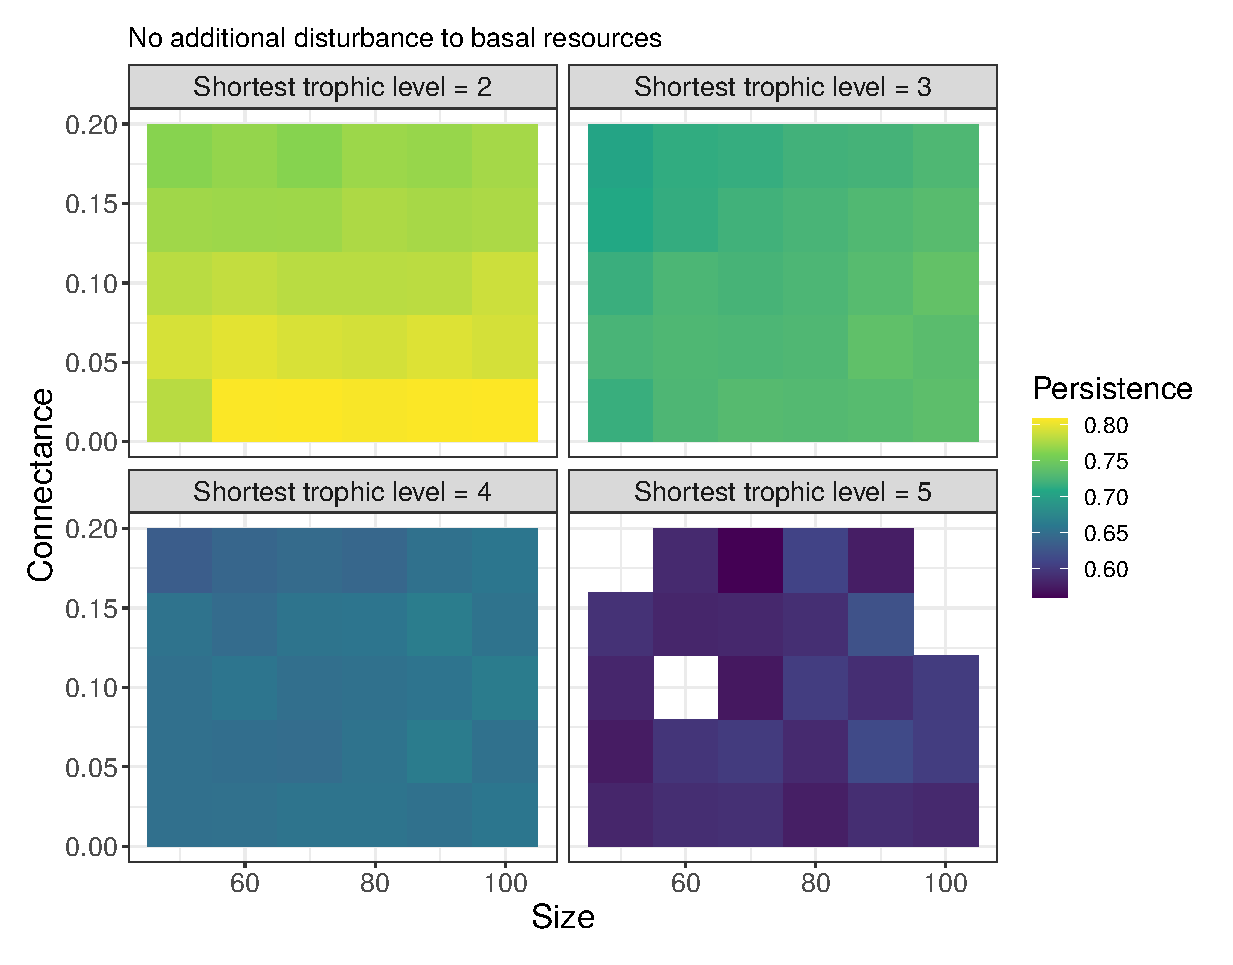
\includegraphics[width=.9\textwidth]{figures/heatmap_STL_allCS_BP0.eps}
    %  \caption{All species across all levels experience a risk of going extinct due to causes not related to the web of $\pi = 0.1$. The panels show final persistence for consumers with different shortest trophic level, for increasing connectance (y-axis) and network size (x-axis). Persistence decreases with darker color in the heat map.}
    %  \label{fig:heatmap_stl_BP0}
    % \end{figure}


    % \begin{figure}[hb!]
    %  \centering
    %  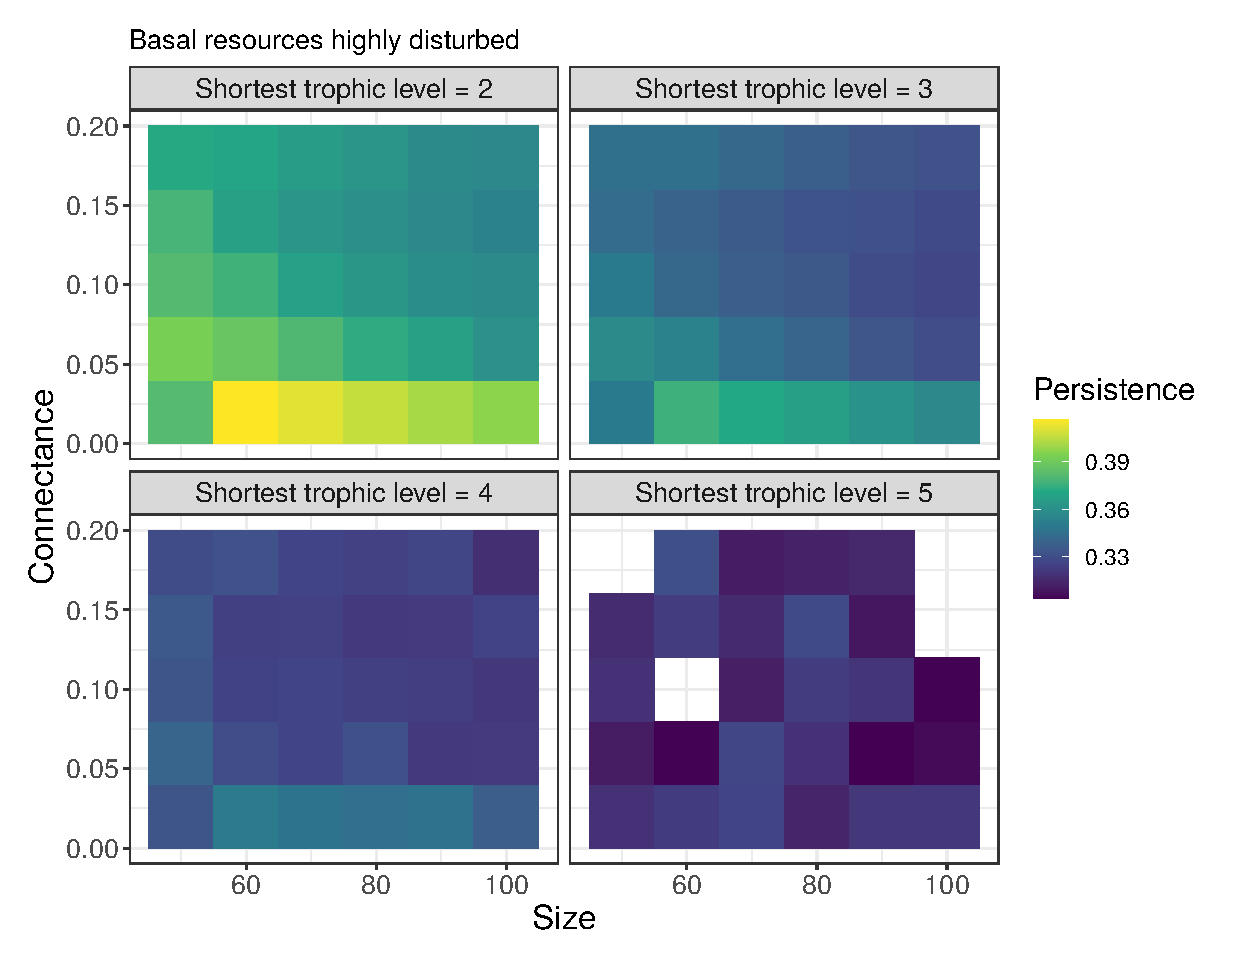
\includegraphics[width=.9\textwidth]{figures/heatmap_STL_allCS_BP1.eps}
    %  \caption{Basal resources experience a disturbance increasing their probability of extinction to $\pi = 0.5$. All consumer species go extinct due to causes not related to the web itself with probability $\pi = 0.1$. The panels show final persistence for consumers with different shortest trophic level, for increasing connectance (y-axis) and network size (x-axis). Persistence decreases with darker color in the heat map.}
    %  \label{fig:heatmap_stl_BP1}
    % \end{figure}

\clearpage

\section{Within-network motif-persistence relationships}

    We compared the outcomes from linear mixed-effect models (GLMMs) relating persistence to motif roles across all networks (Fig. 3 and Table 1, \emph{Main Text}) with similar general linear regressions (GLRs) made on each single network separately.
    The main trends are similar in both analyses, but different-sized networks showed slightly different results for some motifs when considered individually (Figure~\ref{fig:density_prop_S}).
    For the three-species chain and omnivory motifs, a significant interaction between disturbance and the effect of the focal motif means that having a larger proportion of the role be made up of the chain or omnivory motif is associated with lower persistence at high levels of disturbance (Fig. 3 and Table 1, \emph{Main Text}). 
    The same pattern holds overall for GLRs fit within a network  (Figure~\ref{fig:density_prop_S}): the fraction of negative slopes for the proportion of three-species chain and omnivory motifs increases with increasing disturbance. 
    This trend is most pronounced in large networks. (bottom panel, Figure~\ref{fig:density_prop_S}). 
    % Besides the decrease in fraction of positive slopes with increasing disturbance, the omnivory motif showed a higher overall fraction of positive slopes in comparison to the three-species chain motif, corresponding to the positive main effect of omnivory (Fig. 3 and Table 1, \emph{Main Text}). 
    
    
    \begin{figure}[hb!]
        \centering
            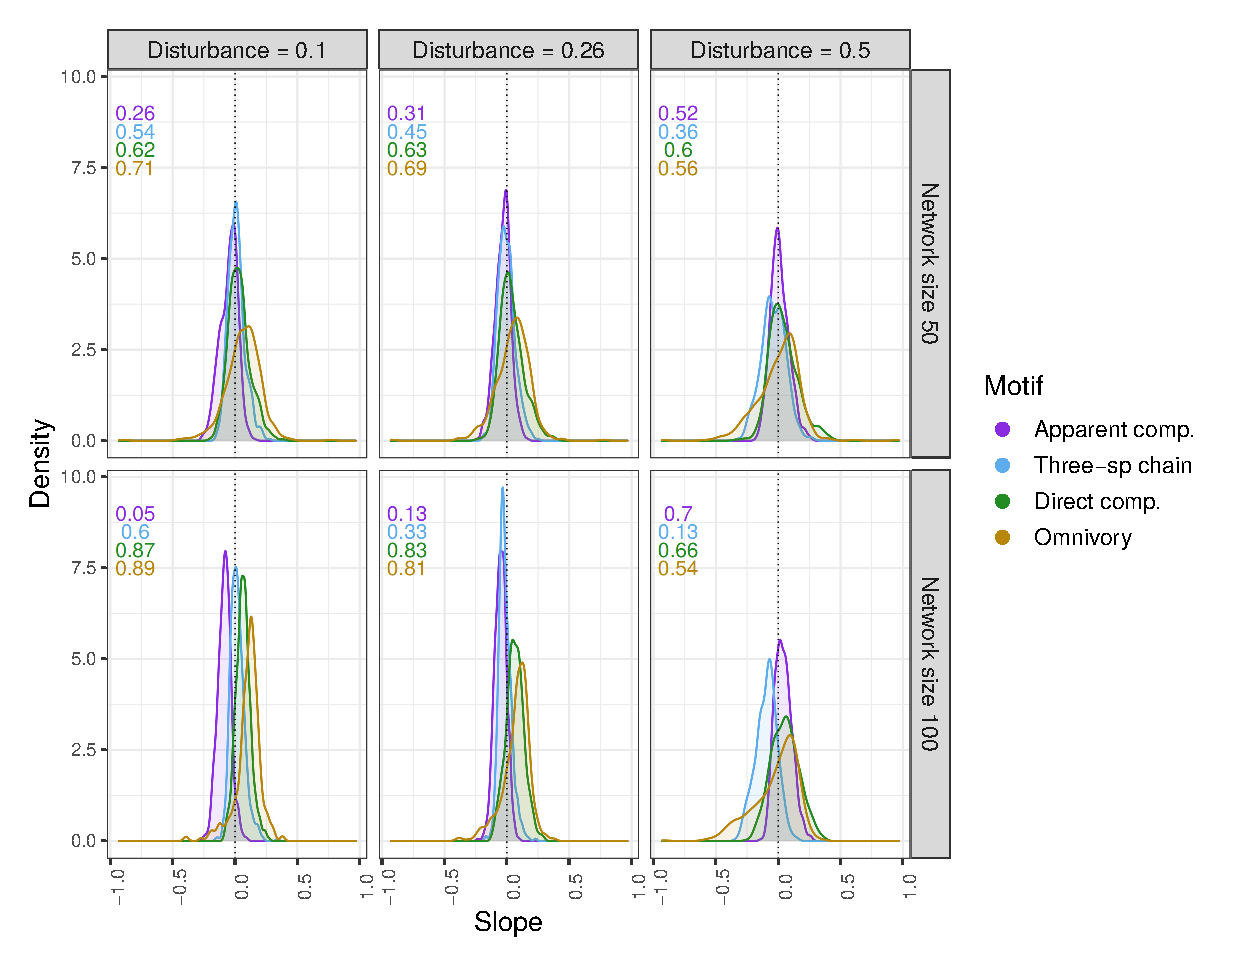
\includegraphics[width=\textwidth]{figures/prop_dens_bp_vs_S_allC.eps}
            \caption{Here we show the density (y-axis) of slopes (x-axis) for regressions of probability of persistence against proportion of different motifs for all simulated webs of all connectances - a visualization of how an increased proportion of each motif (different colored lines) affects the probability of persistence for consumer species. Columns show the result for various disturbances on the basal level, from $\pi = 0.1$ (left) to $\pi = 0.5$ (right). Rows show various network sizes. The dotted, vertical lines indicate zero on the x-axis. A negative slope value reflects a negative relationship between increased participation in a motif and persistence, while a positive slope value reflects a positive relationship - an increased proportion of a specific motif increase persistence. The fraction of replicates with a slope greater than zero are stated in numbers in each sub-plot. Line color corresponds to the motif. }
            \label{fig:density_prop_S}
        \end{figure}    

    
    
    For the apparent and direct competition motifs, the LMMs include a positive interaction between disturbance and the proportion of the motif in a species' role (Fig. 3 and Table 1; \emph{Main Text}).
    This means that having more of the role made up of these two motifs is increasingly beneficial at higher levels of disturbance, a trend which is also evident from the increasing fraction of positive slopes with increasing disturbance based on LRs of each network at each level of disturbance. % (Figure~\ref{fig:density_prop_S}).
    As with the trends for omnivory and three-species chains, these increases are strongest in large networks. % (bottom row, Figure~\ref{fig:density_prop_S}).
    % For direct competition, the fraction of slopes are similar across disturbance levels. Although this interaction is not positive when accounting for network size, the fraction of positive slopes are throughout high.
    The increase in the proportion of positive slopes was much stronger for apparent competition than direct competition, consistent with the smaller (but still significant) interaction term for between direct competition in the LMMs.
    A high proportion of direct competition in a species' role tended to be associated with greater probability of persistence across levels of disturbance and network size.
    % In conclusion, species richness does not considerably alter the trends visible in the LMMs. High species richness more clearly display an interaction between motif proportion, persistences and disturbance levels, while this effect is smaller with low species richness. 
\clearpage
                
\section{Persistence and whole-network motif profiles} [[updated]]

    % Updated and expanded to include permanova tests
    Mean persistence of all consumers varied with the frequencies of different motifs in a network profile ($F_{1,2998}$=645, $p$\textless0.001 for a PERMANOVA of dissimilarity in motif profiles against mean persistence).
    However, motif profiles were not evenly distributed across mean persistences ($F_{134,2865}$=1.77, $p$\textless0.001 for an ANOVA of dissimilarity in motif profiles against mean persistence, rounded to 3 decimal places).
    Specifically, motif profiles were more variable (higher dissimilarities) in networks with higher mean persistence.
    As non-homogeneous variability can cause a PERMANOVA to return a false positive~\citep{Anderson2001}, this means that we must treat our PERMANOVA result as tentative and place more weight on the single-motif regressions.


    % Updated to use mean instead of all species
    \begin{table}[hb!]
        \caption{Coefficients ($\beta$) for models relating persistence to the proportion of a network profile made up by a focal motif, the level of disturbance to basal resources (corresponding to a probability of extinction ranging between 0.1 and 0.5), and their interaction. Coefficients in \textbf{bold} are significant ($\alpha$\textless0.005). Predictors were centered and scaled before model fitting; coefficients refer to a unit increase in predictors. We also provide McFadden's pseudo-$R^2$ value for each regression. }
        \label{motif_profile_tab}
        \centering
        \footnotesize
        \begin{tabular}{c|c c c c c | c }
        Motif & Intercept & Proportion & Disturbance & Interaction &  pseudo-$R^2$ \\
            \hline
            Three-species chain & \textbf{0.326} &  0.0260 & \textbf{-0.595} & -2.53$\times10^{-3}$ & 0.*958 \\
            Apparent competition & \textbf{0.326} & \textbf{0.0501} & \textbf{-0.596} & -2.00$\times10^{-3}$ & 0.962 \\
            Direct competition & \textbf{0.326} & 0.0151 & \textbf{-0.595} & -5.34$\times10^{-4}$ & 0.956 \\
            Omnivory & \textbf{0.326} & \textbf{-0.0626} & \textbf{-0.596} & 3.22$\times10^{-3}$ & 0.966 \\
        \end{tabular}
    \end{table}
\clearpage


\section{Motif profiles and global properties} [[updated]]
    % No update needed

    A network's normalized motif profile (i.e., proportions of the total made up by each motif) was related to the network's size, connectance, and the interaction between them ($F_{1,2996}$=74.3, $p$\textless0.001; $F_{1,2996}$=4203, $p$\textless0.001; and $F_{1,2996}$=27.8, $p$\textless0.001, respectively in a PERMANOVA of dissimilarity in normalized network motif profiles against network size, connectance, and their interaction).
    However, normalized motif profiles were not homogeneously variable across levels of network size, connectance, or their interaction  ($F_{5,2994}$=16.8, $p$\textless0.001; $F_{4,2995}$=31.7, $p$\textless0.001; and $F_{29,2970}$=11.9, $p$\textless0.001 for ANOVAs of dispersion of motif profiles against size, connectance, and combinations of size and connectance, respectively). 
    These differences in variability can cause false positives in the PERMANOVA test. Variability was highest in small and low-connectance networks (Fig.~\ref{dispersion_normmotifs}).
    A series of general linear regressions support the relationship between network motif profiles and global structural properties.
    Specifically, the frequency of the omnivory motif increased in more-connected networks (Table~\ref{network_prop_lms}) while the frequencies of other motifs were not significantly related to network size or connectance.


   \begin{figure}[hb!]
       \centering
       \includegraphics[width=.75\textwidth]{figures/proportion_profile_dispersion.eps}
       \caption{Dispersion of normalized motif profiles (i.e., proportions of each motif) within a network about the centroid for that combination of network size and connectance. Each circle represents a single network; circle colour indicates network size. Scatter has been introduced about each level of connectance to increase visual clarity; the levels of connectance we consider are indicated by vertical black lines.}
       \label{dispersion_normmotifs}
    \end{figure}


     \begin{table}[hb!]
        \centering
        \caption{Coefficients for general linear regressions relating the proportion of each motif in the total motif profile of a network to network size, connectance, and their interaction. Coefficients in \textbf{bold} are significant ($\alpha$\textless0.05). The regression was fit using a binomial error distribution and logit link function.}
       \label{network_prop_lms}
       \begin{tabular}{c|c c c c c}
            Motif & Intercept & Size & Connectance & Interaction \\
            \hline
            Three-species Chain & \textbf{-1.04} & 0.001 & -0.795 & -0.019 \\
            Apparent Competition & 0.168 & -0.002 & -4.09 & 0.010 \\
            Direct Competition & \textbf{-1.42} & -3.69$\times10^{-4}$ & -3.97 & 0.042 \\
            Omnivory & \textbf{-2.99} & 0.003 & \textbf{12.9} & -0.036\\
            \hline
            \end{tabular}
    \end{table}        
\clearpage
    
            

\section{Persistence and global network properties} [updated]

    Connectance had a smaller, but significant, effect on consumer persistence than disturbance (Figs.~\ref{fig:lm_CS}, Table~\ref{tab:per_vs_SC}).
    Network size had no effect on consumer persistence in these simulated networks.

    % updated to use network means rather than all species
    \begin{figure}[hb!]
        \centering
        \includegraphics[width=0.9\textwidth]{figures/persistence_vs_SC_lm.eps}
        \caption{Persistence decreased strongly with increasing probability of disturbance to basal resources and decreased slightly, but significantly, with increasing connectance. The effects of network size and interactions between predictors were not significant. }
        \label{fig:lm_CS}
    \end{figure}



    % \begin{figure}[hb!]
    %     \centering
    %   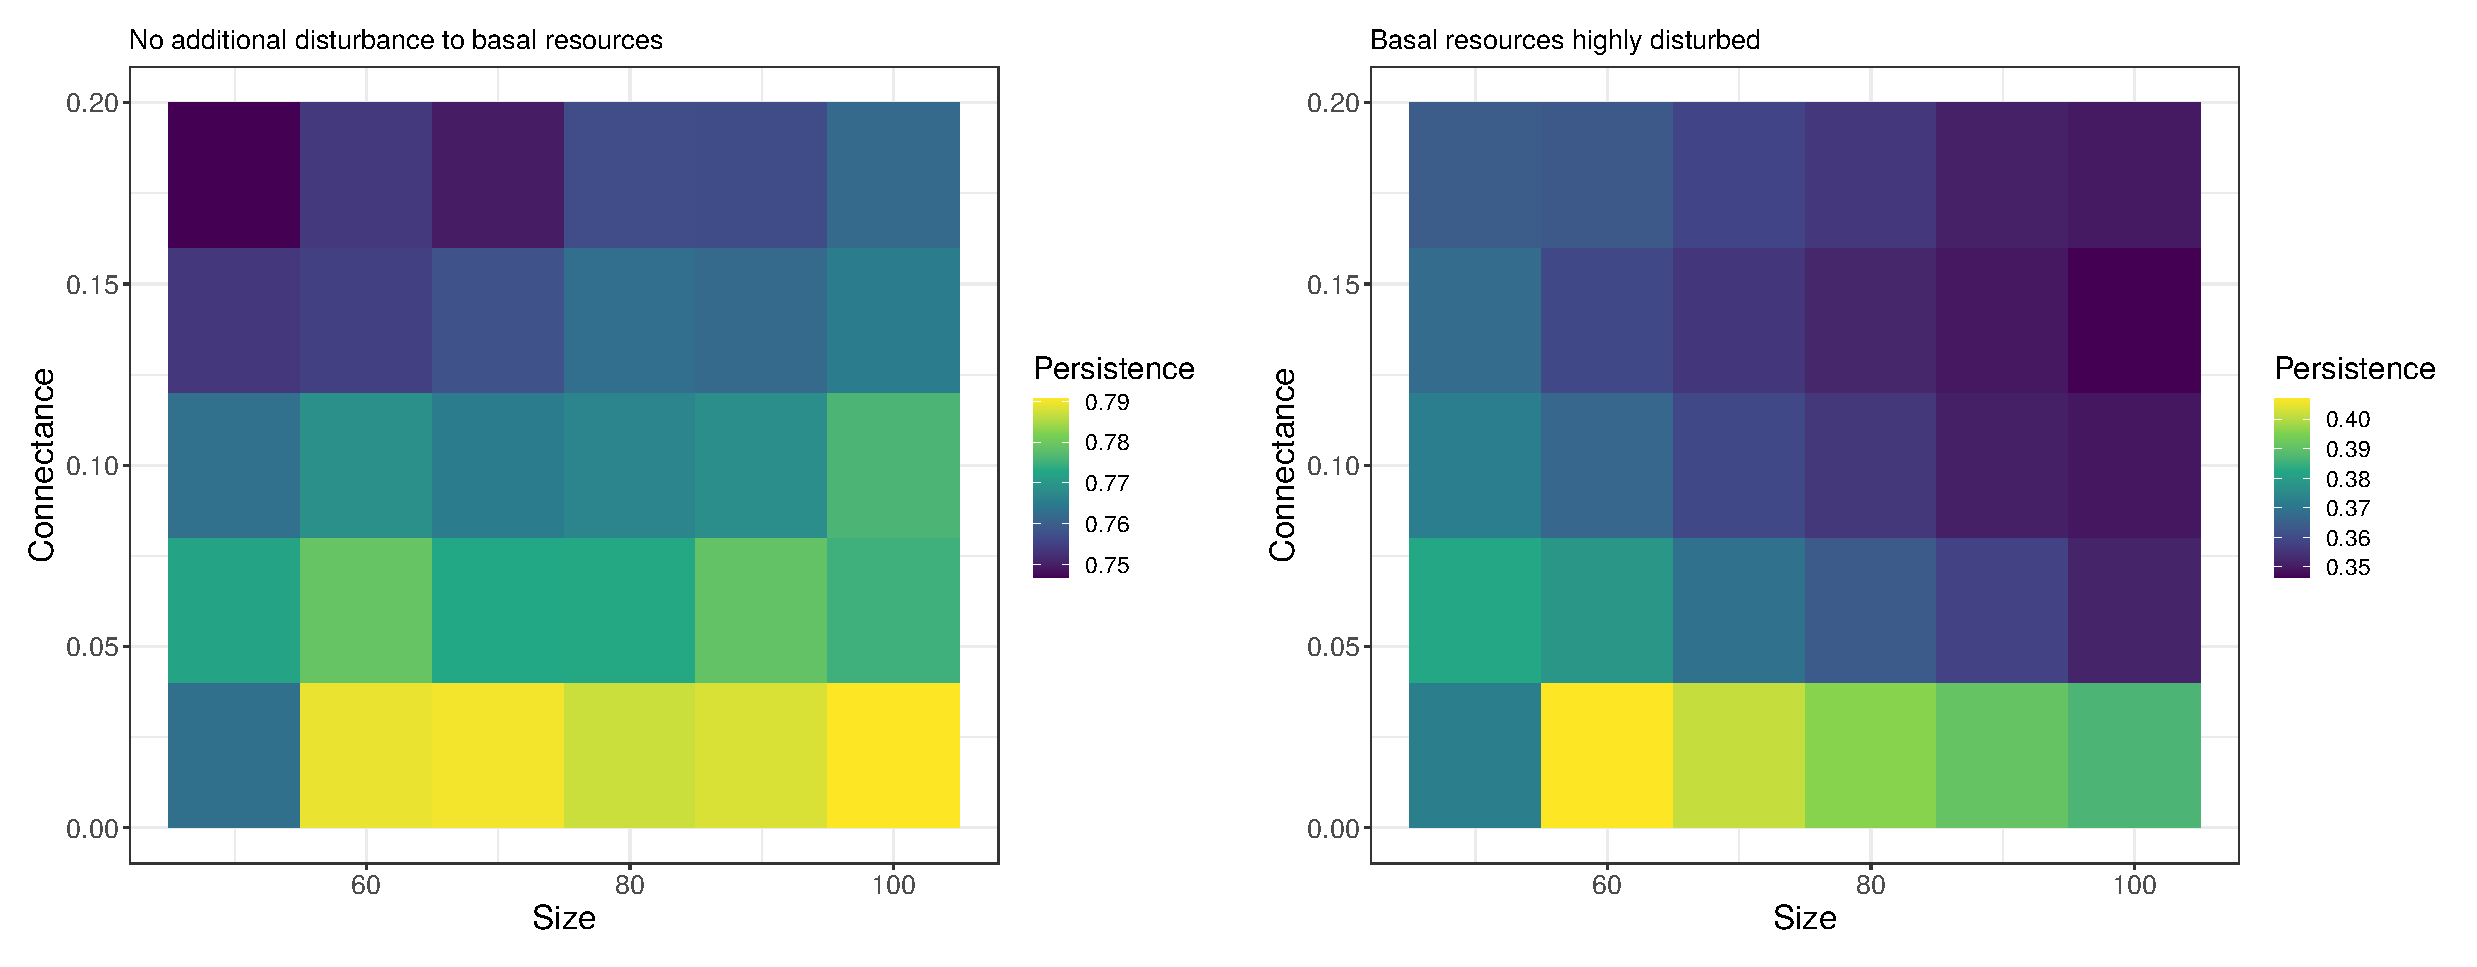
\includegraphics[width=\textwidth]{figures/heatmap_CS_BPcompare.eps}
    %    \caption{Heat maps of average consumer persistence in networks with varying connectance (y-axis) and network size (x-axis) at two levels of disturbance to basal resources. Persistence decreases with darker color in the heat map. When basal species are not disturbed, all species experience a baseline extinction risk of $\pi = 0.1$. When basal species are highly disturbed, their baseline extinction risk rises to $\pi = 0.5$ while the baseline risk of consumers is not changed.}
    %    \label{fig:heatmap_CS}
    % \end{figure}


    % Updated to use mean rather than all species.
    \begin{table}[hb!]
        \caption{Mean persistence of consumers within a network depends on connectance (C) and the level of disturbance to basal resources (D), but not network size (S) or interactions between properties. We show effect sizes ($\beta$) and $p$-values for each coefficient in a general linear model (fit using a binomial error distribution and logic link function). All predictors were centered and scaled before fitting the model. The level of disturbance corresponds to basal resources having a probability of extinction ranging between $0.1 - 0.5$ (see \emph{Methods}). McFadden's pseudo-$R^2$=0.966.
        }
        \label{tab:per_vs_SC}
        \centering
        \begin{tabular}{c|c c |}
            Predictor & $\beta$ & $p$-value \\
            \hline
            Intercept & \textbf{0.326} & \textless0.001 \\
            Size & -7.21$\times10^{-4}$  & 0.964 \\
            Connectance & \textbf{-6.12$\times10^{-2}$}& \textless0.001 \\
            Disturbance & \textbf{-0.596} & \textless0.001 \\
            S:C & -4.48$\times10^{-3}$ & 0.777 \\
            S:D & -1.63$\times10^{-2}$ & 0.316 \\
            C:D & -4.52$\times10^{-3}$ & 0.781 \\
            S:C:D & -1.35$\times10^{-3}$ & 0.934 \\
        \end{tabular}
    \end{table}

\clearpage

\section{Glossary}

 \begin{table}[hb!]
 \label{glossary}
 \caption{Glossary of terms relating to motifs and Bayesian networks}
     \footnotesize{
 \begin{tabular}{l|m{11cm}}
     Term & Definition \\
     \hline
     Global property & A property of the whole network (e.g., species richness) \\
     Local property & A property of a single species, generally referring only to direct interactions (e.g., degree) \\
     Meso-scale property &  A property of a single species which includes direct and indirect interactions; the species' immediate `neighbourhood' in the network (e.g., motif participation) \\
     Motif & Set of $n$ interacting species. In this case, $n=3$ \\
     Network motif profile & Vector describing the frequency of each motif in the network (normalised by dividing counts of each motif by the total participation in  all motifs).\\
     Motif participation role & Vector describing the frequency with which a focal species appears in each motif  (normalised by dividing counts for each motif by the total of all motifs). \\
     Bayesian network & A directed acyclic graph, used to efficiently predict species' likelihood of persistence based on the state of their resources. \\
     Network mean persistence & The mean likelihood of persistence for all consumers in a network.\\
     Species persistence & The likelihood of a particular focal species not going extinct.\\
     In-degree & Number of prey species to a consumer species.\\
     Trophic level (STL) & Length of shortest food chain between the focal species and any basal resource.\\
     Disturbance ($\pi_{disturbed}$) & Probability of extinction of a basal resource after a disturbance is added. \\
     Baseline extinction &  Probability of extinction when no disturbance is applied, $\pi_{base}$=0.1.\\
 \end{tabular}}
 \end{table}
 
\clearpage 

\bibliographystyle{jae} 
\bibliography{anna_bib_new} % Abbreviate journal titles.

\end{spacing}

\end{document}